\documentclass[HS.tex]{subfiles}
\begin{document}

\chapter{Homología simplicial}


\section{Complejo de cadenas simpliciales}
\begin{defi}
Sea $K$ un  complejo simplicial, y $\sigma \in K$ un $n$-símplice (sin pérdida de generalidad) $\sigma = (v_0,v_1,\dots,v_n)$.
Definimos la relación de equivalencia $(v_0,v_1,\dots,v_n) \sim (v_{\pi(0)},v_{\pi(1)},\dots,v_{\pi(n)})$ si $\pi$ es una permutación par de $\{0,1,\dots,n\}$.
\end{defi}
Es decir, la relación de equivalencia inducida por la acción del grupo de las permutaciones pares sobre los $n$-símplices.
Es sencillo ver que esto realmente es una relación de equivalencia.

Mediante esta relación de equivalencia, aparecen dos clases de equivalencia (si $n > 0$, ya que para $n=0$ solo hay una), que llamamos \index{orientación}\emph{orientaciones} sobre $\sigma$, que denotaremos por $\sigma$ y $\overline{\sigma}$.

Cuidado, aquí usamos el mismo símbolo para $\sigma$ el $n$-símplice y $\sigma$ al $n$-símplice orientado.
Escribiremos $(v_0,v_1,\dots,v_n)$ para referirnos a un $n$-símplice y $[v_0,v_1,\dots,v_n]$ para referirnos a un $n$-símplice orientado.

Dado un complejo simplicial $K$, procedemos a definir un complejo de cadenas $\CC(K;F)=\{(C_n(K;\mathbb{F}), \partial_n)\}_{n\geq 0}$. 
\begin{defi}
Definimos $C_n(K;\mathbb{F})$ como el $\mathbb{F}$-espacio vectorial generado por todos los $n$-símplices orientados de $K$ cocientado por el subespacio vectorial $\gene{\sigma + \overline{\sigma} \mid \sigma\ n\text{-símplice de }K}$.
\end{defi}
Por ejemplo, $C_0(K;\mathbb{F})$ es el $\mathbb{F}$-espacio vectorial generado por los vértices de $K$.

\begin{defi}
Definimos los \index{borde}\emph{operador borde} $\partial_n \colon C_n(K; \mathbb{F}) \to C_{n-1}(K; \mathbb{F})$ como un operador lineal generado por:
\[ \partial_n[v_0,v_1,\dots,v_n] := \sum_{i=1}^n (-1)^i [v_0,v_1,\dots,\widehat{v_i},\dots,v_n]\]
\end{defi}

\begin{ej}
\[ \partial_2[v_0,v_1,v_2] = [v_1,v_2] - [v_0,v_2] + [v_0,v_1] = [v_0,v_1] + [v_1,v_2] + [v_2,v_0] \]
\end{ej}

\begin{nota}
Obsérvese que $\partial_0 \colon C_0(K; \mathbb{F}) \to 0$.

En el caso $n=1$, quitaremos los corchetes, es decir $\partial_1[v_0,v_1] = [v_1]-[v_0] = v_1 - v_0$.
\end{nota}

\begin{lemma}
El operador borde $\partial_n \colon C_n(K; \mathbb{F}) \to C_{n-1}(K; \mathbb{F})$ está bien definido.
\end{lemma}
\begin{proof}
Tenemos que ver que si tomamos otro representante de $[v_0,\dots,v_n]$, tenemos la misma imagen.
Basta probar realmente que $\partial([v_0,v_1,\dots,v_n]) = -\partial_n([v_1,v_0,v_2\dots,v_n])$.
\[ \partial([v_0,v_1,\dots,v_n]) = [v_1,v_2,\dots,v_n]-[v_0,v_2,\dots,v_n] + \sum_{i\neq0,1}(-1)^i[v_0,v_1,\dots,\widehat{v_i},\dots,v_n]\]
\[ \partial([v_1,v_0,\dots,v_n]) = [v_0,v_2,\dots,v_n]-[v_1,v_2,\dots,v_n] + \sum_{i\neq0,1}(-1)^i[v_1,v_0,\dots,\widehat{v_i},\dots,v_n]\]
Los dos primeros términos de la primera ecuación son opuestos a los de la segunda. Además, cada término del sumatorio aparece en la otra ecuación con una trasposición en los vértices.
Luego $\partial([v_0,v_1,\dots,v_n]) = -\partial([v_1,v_0,\dots,v_n])$.
\end{proof}

\begin{lemma}
Se tiene que $\partial_n \circ \partial_{n+1} = 0$ para todo $n$.
\end{lemma}
\begin{proof}
\begin{align*}
\partial_n(\partial_{n+1}([v_0,\dots,v_{n+1}])) & = \partial_n \left(\sum_{i=0}^{n+1} (-1)^i [v_0,\dots,\widehat{v_i},v_{n+1}]\right)\\
& = \sum_{i=0}^{n+1} (-1)^i \partial_n([v_0,\dots,\widehat{v_i},v_{n+1}])\\
& = \sum_{i=0}^{n+1} (-1)^i \left(\sum_{j<i} (-1)^j [v_0,\dots,\widehat{v_j},\dots,\widehat{v_i},\dots,v_{n+1}]\right. \\
& \qquad\qquad \left.+ \sum_{j>i} (-1)^{j-1} [v_0,\dots,\widehat{v_i},\dots,\widehat{v_j},\dots,v_{n+1}]\right)
\end{align*}
Si $k < l$, el símplice orientado $[v_0,\dots,\widehat{v_k},\dots,\widehat{v_l},\dots,v_{n+1}]$ aparece dos veces en la combinación lineal anterior: cuando $(i,j)=(l,k)$ y cuando $(i,j)=(k,l)$.
En la primera aparición, tiene signo $(-1)^{k+l}$, en la otra aparición tiene signo $(-1)^{k+l-1}$, luego su suma es $0$.
Como todos los símplices se anulan, tenemos el lema.
\end{proof}

Entonces tenemos el complejo de cadenas simpliciales orientadas en $K$:
\[ \dots \to C_{n+1}(K; \mathbb{F}) \xrightarrow{\partial_{n+1}} C_n(K; \mathbb{F}) \xrightarrow{\partial_n} C_{n-1}(K; \mathbb{F}) \to \dots \to C_0(K; \mathbb{F}) \to 0 \]
De aquí podemos definir el $n$-ésimo espacio vectorial de homología simplicial de $K$ (todos sus símplices con el mismo signo de orientación):
\[ H_n(K; \mathbb{F}) := \frac{\ker \partial_n}{\Ima \partial_{n+1}}\]


\begin{prop}
El complejo de cadenas $\{(C_n(K;\F),\partial_n)\}_{n\geq 0}$ admite un aumento siempre que $K\neq \emptyset$.
\end{prop}

\begin{dem}
Hay que buscar $\varepsilon:C_0(K;\F)\to\F$ homomorfismo sobreyectivo tal que $\varepsilon\circ\partial_1=0$. Basta tomar la aplicación $v\mapsto \varepsilon(v)=1$ para todo vértice $v\in K$. Claramente es un homomorfismo sobreyectivo. También es fácil ver que $\varepsilon\circ\partial_1=0$, pues
\[
\varepsilon(\partial_1[v_i,v_j])=\varepsilon(v_i-v_j)=\varepsilon(v_i)-\varepsilon(v_j)=1-1=0
\]
\QED
\end{dem}
El complejo
\[
\cdots\to C_{n+1}(K;\F)\overset{\overline{\partial}_{n+1}}{\to}C_n(K;\F)\overset{\overline{\partial}_n}{\to}\cdots\to C_0(K;\F)\overset{\varepsilon}{\to}\F\to 0
\]
da lugar a la homología simplicial reducida dada por 
\[
\widetilde{H}_n(K;\F)=\frac{\ker\overline{\partial}_n}{\Ima\overline{\partial}_{n+1}}
\]
donde $\overline{\partial}_0=\varepsilon$. Recordemos que $\widetilde{H}_n(K;\F)=H_n(K;\F)$ cuando $n\neq 0$ y $H_0(K;\F)=\widetilde{H}_0(K;\F)\oplus\F$.

\begin{prop}
Sean $K$ y $L$ complejos simpliciales y sea $\varphi:K\to L$ una aplicación simplicial. Entonces $\varphi$ induce homomorfismos $\varphi_*:C_n(K;\F)\to C_n(L;\F)$ para todo $n\geq 0$. Es más, se tienen diagramas conmutativos
\[
\begin{tikzcd}
C_n(K;\F)\arrow[r, "\varphi_*"]\arrow[d, "\partial_n"] & C_n(L;\F)\arrow[d, "\partial_n"]\\
C_{n-1}(K;\F)\arrow[r, "\varphi_*"] & C_{n-1}(L;\F)
\end{tikzcd}
\]
En particular, $Id_*=Id$ y $(\psi\circ\varphi)_*=\psi_*\circ\varphi_*$.
\end{prop}
\begin{dem}
Dado $n>0$, definimos $\varphi_*:C_n(K;\F)\to C_n(L;\F)$ de la siguiente manera
\[
\varphi_*([v_0,\dots, v_n])=\begin{cases}
[\varphi(v_0), \dots, \varphi(v_n)] & \varphi(v_i)\neq\varphi(v_j)\forall i\neq j\\
0& c.c.
\end{cases}
\]
Si $(v_0,\dots, v_n)$ es un $n$-símplice de $K$ entonces su imagen es un símplice de $L$ por ser $\varphi$ simplicial. Esta aplicación está bien definida además por la definición de las clases de equivalencia. Veamos la conmutatividad. Supongamos que tenemos un símplice con todos sus vértices distintos entre sí:
\[
\partial_n(\varphi_*([v_0,\dots, v_n]))=\partial_n([\varphi(v_0), \dots, \varphi(v_n)])=
\]
\[
\sum_{i=0}^n(-1)^i[\varphi(v_0), \dots,\widehat{\varphi(v_i)},\dots,  \varphi(v_n)]=\sum_{i=0}^n(-1)^i\varphi_*([v_0,\dots, \hat{v}_i,\dots, v_n])=
\]
\[
\varphi_*\left(\sum_{i=0}^n(-1)^i[v_0,\dots, \hat{v}_i,\dots, v_n]\right)=\varphi_*(\partial_n[v_0,\dots, v_n])
\]

Por otro lado, si algún vértice se repite, es decir, $\varphi(v_i)=\varphi(v_j)$ para algún $i\neq j$ (supondremos por sencillez que solo en un caso), entonces $\partial_n(\varphi_*([v_0,\dots, v_n]))=0$. Mientras que
\[
\varphi_*(\partial_n[v_0,\dots, v_n])=\varphi_*\left(\sum_{k=0}^n(-1)^k[v_0, \dots, \hat{v}_k,\dots, v_n]\right)=\sum_{k=0}^n(-1)^k\varphi_*([v_0,\dots, \hat{v}_k,\dots, v_n])
\]
Para todo $k\neq i,j$ se tiene que $\varphi_*[v_0,\dots, \hat{v}_k,\dots, v_n]=0$, así que la suma anterior nos da
\[
(-1)^i\varphi_*[v_0,\dots, \hat{v}_i,\dots, v_n]+(-1)^j\varphi_*([v_0,\dots, \hat{v}_j,\dots, v_n])=
\]
\[
(-1)^i[\varphi(v_0),\dots, \widehat{\varphi(v_i)},\dots, \varphi(v_n)]+(-1)^j[\varphi(v_0),\dots, \widehat{\varphi(v_j)},\dots, \varphi(v_n)]
\]
Pongamos que $i<j$ sin pérdida de generalidad. Entonces
\[
[\varphi(v_0),\dots, \widehat{\varphi(v_i)},\dots, \varphi(v_n)]=(-1)^{j-i-1}[\varphi(v_0),\dots, \widehat{\varphi(v_j)},\dots, \varphi(v_n)]
\]
y al sustituir obtenemos 0, como deseábamos. La functorialidad se deduce directamente de la definición.
\QED
\end{dem}

\begin{ej}\
\begin{enumerate}
\item \underline{Homología de un vértice (0-símplice)}: si $K=\{v\}$, su complejo de cadenas asociado es trivial en todos los niveles salvo en $C_0(K)=\gene{v}$. Por tanto, $H_q(K)=0$ para todo $q\geq 1$ y $H_0(K)=\frac{\ker\partial_0}{\Ima\partial_1}=\ker\partial_0=\gene{v}\cong\F$. Se tiene entonces que $\dim H_0(K)=1$ y en el resto de casos $\dim H_q(K)=0$. A estos números se los llama \emph{números de Betti}. En el caso de la homología reducida, $\widetilde{H}_0=\frac{\ker\varepsilon}{\Ima\partial_1}=\ker\varepsilon=0$. 

\item \underline{Homología de un cono}: Sea $K=vL$ un cono simplicial. Tenemeos la inclusión natural $i:\{v\}\to K$, que induce una aplicación $i_*: \{(C_n,\partial_n)\}\to \{(C_n(K),\partial_n)\}$. La idea es probar que $i_*$ induce una equivalencia de homotopía entre los complejos de cadenas. Sea $g:\{(C_n(K),\partial_n)\}\to \{C_n(v),\partial_n)\}$ definida como $g_n(\sigma)=0$ para $n\geq 1$ y $g_0(v_i)=v$ para todo $v_i\in K^0$. Es claro que $g\circ i_*=Id_{\CC(v)}$. Vamos a ver que $i_*\circ g\simeq Id_{\CC(K)}$. Definimos una homotopía $h: \CC(K)\to\CC(K)[+1]$ como 
\[
h_n ([v_0,\dots,v_n]) = \begin{cases}
	[v, v_0,\dots,v_n] & \text{ si }v_i \neq v\text{ para todo }i\\
	0 & \text{ si existe }i_0\text{ con }v_{i_0} = v
\end{cases}
\]

\[
\begin{tikzcd}
& C_n(K)\arrow[r, "\partial_n"]\arrow[ld, "h_n" above]\arrow[d, shift left, "Id_n" left=5pt]\arrow[d, shift right, "i_{*n} \circ g_n" right=5pt] & C_{n-1}(K)\arrow[ld, "h_{n-1}"]\\
C_{n+1}(K)\arrow[r, "\partial_{n+1}"] & C_n(K)
\end{tikzcd}
\]

Sea $σ$ un $n$-símplice de $K$ con $n\geq 1$. Si $σ$ no contiene $v$, entonces:
\[  Id_n([v_0,\dots,v_n])- i_{*n} \circ g_n ([v_0,\dots,v_n])=  Id_n(v_0,\dots,v_n) -0= [v_0,\dots,v_n] \]
\begin{align*}
(\partial_{n+1} \circ h_n & + h_{n-1} \circ \partial_n)(v_0,\dots,v_n) = \partial_{n+1}([v,v_0,\dots,v_n]) + h_{n-1}\left(\sum_{i=0}^n (-1) [v_0,\dots,\widehat{v_i},\dots,v_n]\right)\\
& = [v_0,\dots, v_n]+\sum_{i=0}^n (-1)^{i+1} [v,v_0,\dots,\widehat{v_i},\dots,v_n] + \sum_{i=0}^n(-1)^i h_{n-1}[v_0,\dots,\widehat{v_i},\dots,v_n]\\
& = [v_0,\dots,v_n] + \sum_{i=0}^n (-1)^{i+1} [v,v_0,\dots,\widehat{v_i},\dots,v_n] + \sum_{i=0}^n (-1)^{i} [v,v_0,\dots,\widehat{v_i},\dots,v_n]\\
& = [v_0,\dots,v_n]
\end{align*}
Si por el contrario, $σ$ contiene un vértices $v_{i_0}=v$ tenemos que:
\[  Id_n([v_0,\dots,v_n])-i_{*n} \circ g_n ([v_0,\dots,v_n]) =  Id_n([v_0,\dots,v_n])-0 = [v_0,\dots,v_n] \]
Como $h_n([v_0,\dots,v_n])=0$ ahora:
\begin{align*}
(\partial_{n+1} \circ h_n & + h_{n-1} \circ \partial_n)[v_0,\dots,v_n] =  h_{n-1}(\partial_n[v_0,\dots,v_n])\\
& = h_{n-1}\left(\sum_{i=0}^n (-1)^i [v_0,\dots,\widehat{v_i},\dots,v_n]\right)\\
& = \sum_{i=0}^n (-1)^i h_{n-1}[v_0,\dots,\widehat{v_i},\dots,v_n]\\
& = (-1)^{i_0}[v,v_0,\dots,\widehat{v_{i_0}},\dots,v_n] \\
& = [v_0,\dots,v_n]
\end{align*}


Para el caso $n=0$, si $v_i\neq v$ entonces $\partial_1h_0([v_i])=\partial_1([v,v_i])=v_i-v=(Id_0-g_0)([v_i])$ y si $v_i=v$, entonces ambos términos son 0, por lo que finalmente se tiene la equivalencia de homotopía.

Esto demuestra que:
\[ H_n(vL) = \begin{cases}
0 & \text{ si }n ≥ 1\\
\gene{v} & \text{ si }n=0
\end{cases}\]
\[ \widetilde{H_n}(vL) = 0 \]

En particular, este resultado es válido para cualquier $n$-símplice, a partir de lo cual podemos calcular los siguiente.

\item \underline{Homología del interior de un $n$-símplice}: podemos evitar el caso $n=0$ por ser el interior de un vértice igual a sí mismo. Si $n=1$ entonces el interior de un segmento son dos vértices, por lo que claramente su homología se obtiene como suma directa de la de los vértices individuales (no así en la reducida, donde la suma directa sería siempre trivial pero la homología reducida de dos vértices es $\F$ en el nivel 0). Para $n\geq 2$ vamos a denotar $\overline{\partial}$ a los operadores borde correspondientes $C_q(\mathring{\sigma})$ y sin la barra a los de $\sigma$. Obsérvese que $C_q(\mathring{\sigma})=C_q(\sigma)$ para $q\leq n-1$ y $C_q(\mathring{\sigma})=0$ para $q\geq n$. De aquí se deduce que la homología $H_q(\mathring{\sigma})=H_q(\sigma)$ para todo $q\leq n-2$ y para $q\geq n$. Ahora bien, $H_{n-1}(\mathring{\sigma})=\ker\overline{\partial}_{n-1}$ pues $\Ima\overline{\partial}_n=0$. Por otra parte, por ser la homología de $\sigma$ trivial en este nivel, se tiene que $\ker\overline{\partial}_{n-1}=\ker\partial_{n-1}=\Ima\partial_n$. Obsérvese que $\partial_n$ es inyectiva, por lo que $\Ima\partial_n\cong \gene{\sigma}\cong\F$, con lo cual ya tenemos la homología que faltaba. 
\end{enumerate}
\end{ej}

\begin{prop}\label{arista}
Sea $σ=(v,w)$ un $1$-símplice
\[ H_n(\partial σ) = \begin{cases}0 & \text{ si }n≥1\\ \F^2\gene{v,w} & \text{ si }n=0\end{cases}\]
\[ \tilde{H}_n(\partial σ) = \begin{cases}0 & \text{ si }n≥1\\ \F\gene{v-w} & \text{ si }n=0\end{cases}\]
\end{prop}
\begin{dem}
Tenemos la sucesión:
\[ \begin{tikzcd}
0 \arrow[r,"\partial_2"] & 0 \arrow[r,"\partial_1"] & {C_0(\partial σ) = \F^2\gene{v,w}} \arrow[rr,"\partial_0"] \arrow[dr,"\varepsilon"] & & 0\\
& & & \F \arrow[ur]
\end{tikzcd}\]
Entonces $H_n(\partial σ) = \frac{\ker \partial_n}{\Ima \partial_{n+1}} = 0$ para todo $n \geq 1$.
Para $n=0$, como $\Ima \partial_1 = 0$, tenemos que $H_0(\partial σ) = \ker \partial_0  = \F^2\gene{v,w}$.
Por otro lado, como $\varepsilon(v)=1$ y $\varepsilon(w)=1$, se deduce que $\ker \varepsilon = \F\gene{v-w}$, luego:
\[ \tilde{H}_0(\partial σ) = \frac{\ker \varepsilon}{\Ima \partial_1} = \ker \varepsilon = \F\gene{v-w} \]
\[ \tilde{H}_n(\partial σ) = H_n(\partial σ) \quad \forall n ≥ 1 \]
\QED
\end{dem}

\begin{prop}
Sea $σ$ un $n$-símplice con $n≥2$ y sea $v \in σ$
\[ H_q(\partial σ) = \begin{cases}
  0 & \text{ si }q \neq n-1,0\\
  \F\gene{\partial_n σ} & \text{ si }q=n-1\\
  \F\gene{v} & \text{ si }q=0\end{cases}\]
\end{prop}
\begin{dem}
\[ \cdots \to 0 \xrightarrow{\partial_n} C_{n-1}(\partial σ) \xrightarrow{\partial_{n-1}} \cdots \xrightarrow{\partial_1}C_0(\partial σ) \xrightarrow{\partial_0} 0
\]
Como $C_q(\partial σ) = C_q(σ)$ para todo $q ≤ n-1$, entonces $H_q(\partial σ) = H_q(σ)$ para todo $q ≤ n-2$.
En consecuencia:
\[ H_q(\partial σ) = \begin{cases} 
  0 & \text{ si }q≤n-2\text{ y }q \neq 0\\
  \F\gene{v} & \text{ si }q=0\end{cases}\]
Por otro lado:
\[ H_{n-1}(\partial σ) = \frac{\ker \partial_{n-1}}{\Ima \hat{\partial}_{n}} = \ker \partial_{n-1}\]
Pero:
\[ H_{n-1}(σ) = 0 \Rightarrow \ker_{\partial_{n-1}} = \Ima \partial_n \]
Tomando $σ = (v_0,\dots,v_n)$.
Como $C_n(σ) = \F\gene{σ}$, entonces:
\[ \Ima \partial_n = \F\gene{\partial_n(σ)} = \F\gene{\sum_{i=0}^n (-1)^i (v_0,\dots,\widehat{v_i},\dots,v_n)}\]
\QED
\end{dem}

\section{Homología relativa}
\begin{defi}
Sea $K$ un complejo simplicial y $L\subseteq K$ un subcomplejo. Entonces el complejo de cadenas $\{C_n(L;\F),\partial_n|\}$ es un subcomplejo de $\{C_n(K;\F),\partial_n\}$ y se llama \emph{homología orientada relativa del par} $(K,L)$ a la homología del \emph{complejo de cadenas relativas}
\[
C_*(K,L;\F)=\{C_n(K,L;\F),\tilde{\partial}_n\}=\{C_n(K,\F)/C_n(L,\F),\tilde{\partial}_n\}
\]
donde $\tilde{\partial}_n$ es el paso al cociente del operador borde. 
\end{defi}

\begin{prop}
Si $L$ es un subcomplejo de $K$ se tiene la sucesión exacta de homología simplicial orientada de $(K,L)$
\[
\cdots\to H_n(L;\F)\overset{i_*}{\to} H_n(K;\F)\overset{j_*}{\to} H_n(K,L;\F)\overset{\Delta}{\to} H_{n-1}(L;\F)\to\cdots
\]
\end{prop}
\begin{dem}
Se sigue al considerar la sucesión exacta de complejos de cadenas
\[
0\to \CC(L;\F)\overset{i}{\to} \CC(K;\F)\overset{j}{\to} \CC(K,L;\F)\to 0
\]
donde $i$ es la inclusión canónica y $j$ es la proyección natural. Basta entonces aplicar la sucesión exacta larga en homología.  \QED
\end{dem}

\begin{nota}
Si consideramos los complejos aumentados $\widetilde{C}_n(K)$ y $\widetilde{C}_n(L)$ obtenemos que el complejo relativo con aumento coincide con el complejo relativo original y tenemos análogamente la sucesión exacta de homología simplicial orientada reducida
\[
\cdots\to \widetilde{H}_n(L;\F)\overset{i_*}{\to} \widetilde{H}_n(K;\F)\overset{j_*}{\to} H_n(K,L;\F)\overset{\Delta}{\to} \widetilde{H}_{n-1}(L;\F)\to\cdots
\]
\end{nota}

\begin{prop}
Si $\sigma$ es un $n$-símplice ($n\geq 1$) se tiene
\[
H_p(\sigma,\mathring{\sigma};\F)\cong\begin{cases}
\F & p=n\\
0 & c.c.
\end{cases}
\]
\end{prop}

La demostración es muy sencilla y se deja como ejercicio. 

\begin{prop}
Sea $K$ un complejo simplicial y $K_1$ y $K_2$ subcomplejos de $K$. Entonces existe una sucesión exacta (\emph{sucesión de Mayer-Vietoris}):
\[
\cdots\to H_n(K_1\cap K_2;\F)\overset{\varphi}{\to}H_n(K_1;\F)\oplus H_n(K_2;\F)\overset{\psi}{\to}H_n(K_1\cup K_2;\F)\overset{\Delta}{\to}H_{n-1}(K_1\cap K_2;\F)\to\cdots
\]
donde $\varphi(x)=(i_{1*}(x),-i_{2*}(x))$ y $\psi(x)=j_{1*}(x)+j_{2*}(x)$, siendo $i_t:K_1\cap K_2\to K_t$ y $j_t:K_t\to K_1\cup K_2$  ($t=1,2$) las correspondientes inclusiones.
\end{prop}

\begin{dem}
Tenemos la sucesión de Mayer-Vietoris para complejos de cadenas
\[
\cdots\to H_n(\mathcal{C}_1\cap\mathcal{C}_2)\overset{\varphi}{\to}H_n(\mathcal{C}_1\oplus\mathcal{C}_2)\overset{\psi}{\to}H_n(\Ima{j})\overset{\Delta}{\to}H_{n-1}(\mathcal{C}_1\cap\mathcal{C}_2)\to\cdots
\]
donde $\mathcal{C}_i=\{C_n(K_i;\F),\partial_n\}$ ($i=1,2$). Obsérvese que $\CC_1\cap\CC_2=\CC(K_1\cap K_2;\F)$. Además $\Ima{j}=\CC(K_1\cup K_2;\F)$ pues trivialmente $\Ima{j_n}\subseteq C_n(K_1\cup K_2;\F)$ y recíprocamente, si $\sigma\in K_1$ entonces $j(\sigma,0)=\sigma$ y análogamente si $\sigma\in K_2$. 
\QED
\end{dem}

\begin{nota}
La sucesión de Mayer-Vietoris también es válida para la homología reducida cuando ninguno de los complejos que intervienen son vacíos.
\end{nota}
\section{Ejemplos de cálculos de homología}
\begin{ej}\label{colapso}
Vamos a calcular la homología de un colapso elemental (la cual se generaliza fácilmente a la de un colapso completo). Sea $K$ un complejo simplicial y $L\subseteq K$ un subcomplejo tal que $K\searrow L=K-\{\sigma,\tau\}$ con $\tau<\sigma$ una cara libre. Aplicamos la sucesión de Mayer-Vietoris para $K_1=L$ y $K_2=\sigma$. 
Como $τ$ es cara libre de $σ$, $σ$ es de hecho un cono sobre $τ$.
Entonces $K_1\cap K_2$ es el cono sobre $\partial\tau$, así que todas las homologías de $K_1\cap K_2$ son triviales.
Entonces tenemos las sucesiones exactas:
\[ 0 \xrightarrow{φ} H_n(L) \oplus H_n(σ) \xrightarrow{ψ} H_n(K) \xrightarrow{Δ} 0 \]
Entonces $ψ$ es un isomorfismo, luego $H_n(K) \cong H_n(L) \oplus H_n(σ)$.
Además para $n\neq 0$, $H_n(σ) = 0$, luego tenemos que $H_q(K) \cong H_n(L)$.

Para $n=0$, consideramos la misma sucesión pero obteniéndola de la sucesión de Mayer-Vietoris para homología reducida, de manera que $\tilde{H_0}(K_1 \cap K_2) = 0$.
\[ 0 \xrightarrow{φ} H_1(L) \xrightarrow{ψ} H_1(K) \xrightarrow{Δ} \tilde{H_0}(K_1 \cap K_2) \]
\end{ej}

\begin{ej}
\begin{enumerate}
\item \underline{Homología del cilindro}:
\begin{figure}[H]
\centering
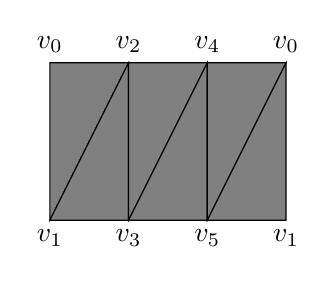
\begin{tikzpicture}
\draw[fill=gray] (0,2) node[anchor=south]{$v_0$} -- (0,0) node[anchor=north]{$v_1$} -- (1,2) node[anchor=south]{$v_2$} -- cycle;
\draw[fill=gray] (0,0) -- (1,2) -- (1,0) node[anchor=north]{$v_3$} -- cycle;
\draw[fill=gray] (1,2) -- (1,0) -- (2,2) node[anchor=south]{$v_4$} -- cycle;
\draw[fill=gray] (1,0) -- (2,2) -- (2,0) node[anchor=north]{$v_5$} -- cycle;
\draw[fill=gray] (2,0) -- (2,2) -- (3,2) node[anchor=south]{$v_0$} -- cycle;
\draw[fill=gray] (2,0) -- (3,2) -- (3,0) node[anchor=north]{$v_1$} -- cycle;
\end{tikzpicture}
\begin{tikzpicture}
\draw (0,1) node[anchor=south]{$\searrow\!\!\searrow$};
\draw (0,0) node[anchor=south]{};
\end{tikzpicture}
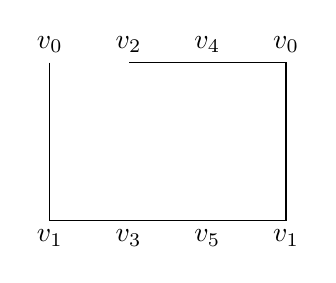
\begin{tikzpicture}
\draw (0,2) node[anchor=south]{$v_0$} -- (0,0) node[anchor=north]{$v_1$} -- (1,0) node[anchor=north]{$v_3$}
-- (2,0) node[anchor=north]{$v_5$} -- (3,0) node[anchor=north]{$v_1$} -- (3,2) node[anchor=south]{$v_0$}
-- (2,2) node[anchor=south]{$v_4$} -- (1,2) node[anchor=south]{$v_2$};
\end{tikzpicture}
\begin{tikzpicture}
\draw (0,1) node[anchor=south]{$\searrow\!\!\searrow$};
\draw (0,0) node[anchor=south]{};
\end{tikzpicture}
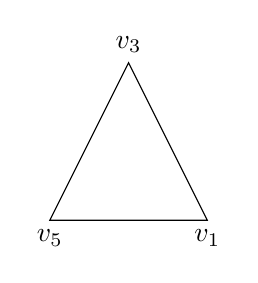
\begin{tikzpicture}
\draw (1,2) node[anchor=south]{$v_3$} -- (0,0) node[anchor=north]{$v_5$} -- (2,0) node[anchor=north]{$v_1$} -- cycle;
\end{tikzpicture}
\end{figure}

Luego:
\[ H_n(K) \cong H_n((v_1,v_5,v_3)) = \begin{cases}
  \F\gene{v_1} & \text{ si }n=0\\
  \F\gene{\partial(v_1,v_5,v_3)} & \text{ si }n=1\\
    0 & \text{ si }n>1\end{cases}\]

\item \underline{Homología de la cinta de Möbius}:
\begin{figure}[H]
\centering
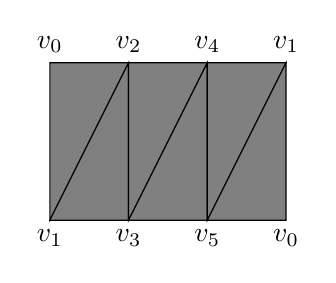
\begin{tikzpicture}
\draw[fill=gray] (0,2) node[anchor=south]{$v_0$} -- (0,0) node[anchor=north]{$v_1$} -- (1,2) node[anchor=south]{$v_2$} -- cycle;
\draw[fill=gray] (0,0) -- (1,2) -- (1,0) node[anchor=north]{$v_3$} -- cycle;
\draw[fill=gray] (1,2) -- (1,0) -- (2,2) node[anchor=south]{$v_4$} -- cycle;
\draw[fill=gray] (1,0) -- (2,2) -- (2,0) node[anchor=north]{$v_5$} -- cycle;
\draw[fill=gray] (2,0) -- (2,2) -- (3,2) node[anchor=south]{$v_1$} -- cycle;
\draw[fill=gray] (2,0) -- (3,2) -- (3,0) node[anchor=north]{$v_0$} -- cycle;
\end{tikzpicture}
\begin{tikzpicture}
\draw (0,1) node[anchor=south]{$\searrow\!\!\searrow$};
\draw (0,0) node[anchor=south]{};
\end{tikzpicture}
\begin{tikzpicture}
\draw (0,2) node[anchor=south]{$v_0$} -- (0,0) node[anchor=north]{$v_1$} -- (1,0) node[anchor=north]{$v_3$}
-- (2,0) node[anchor=north]{$v_5$} -- (3,0) node[anchor=north]{$v_0$} -- (3,2) node[anchor=south]{$v_1$};
\end{tikzpicture}
\begin{tikzpicture}
\draw (0,1) node[anchor=south]{$=$};
\draw (0,0) node[anchor=south]{};
\end{tikzpicture}
\begin{tikzpicture}
\draw (0,2) node[anchor=south]{$v_0$} -- (0,0) node[anchor=north]{$v_1$} -- (2,0) node[anchor=north]{$v_4$} -- (2,2) node[anchor=south]{$v_5$} -- cycle;
\end{tikzpicture}
\end{figure}
Vamos a probar aprovechando este ejemplo, que la homología de cualquier triangulación de la circunferencia como un polígono de $n$ lados es siempre la misma, por lo que tendremos que la homología de la banda de Möbius es la misma que la del cilindro. Sea entonces $K$ una tal triangulación formada por vértices $v_0,\dots, v_{n-1}$. Consideramos los subcomplejos $K_1=K-(v_0,v_1)$ y $K_2=\{v_0,v_1,(v_0,v_1)\}$. Claramente $K_1\cup K_2=K$ y además $K_1\cap K_2=\partial(v_0,v_1)$, por lo que su homología viene dada por la proposición \ref{arista}. Por otro lado, es fácil comprobar que tanto $K_1$ como $K_2$ son colapsables (colapsan sobre un punto), así que por el ejemplo \ref{colapso} tenemos que su homología reducida es trivial. Además es claro que para $n\geq 2$ la homología de esta triangulación es trivial. Así pues, nos vamos a la sucesión de Mayer-Vietoris reducida:
\[
\begin{tikzcd}
 H_1(K_1)\oplus H_1(K_2)\arrow[d,equal]\arrow[r] & H_1(K)\arrow[r] & \widetilde{H}_0(K_1\cap K_2)\arrow[d,equal]\arrow[r] & \widetilde{H}_0(K_1)\oplus \widetilde{H}_0(K_2)\arrow[d,equal]\\
                    0                              &                 &  \F\gene{v_1-v_0} & 0
\end{tikzcd}
\]
Por lo que $\widetilde{H}_1(K)\cong\F$. Luego: $\widetilde{H}_1(K)=\F\gene{z}$, donde $z$ es un $1$-ciclo de $K$ (el único posible es $(v_0,v_1)+(v_1,v_2)+\dots+(v_{n-1},v_0)$).
También tenemos de forma similar que $\widetilde{H}_0(K)=0$, con lo que se tiene el resultado. 
\end{enumerate}
\end{ej}

\begin{defi}
Dados dos complejos simpliciales $K$ y $K'$, se define el \index{wedge}wedge o unión por un punto de $K$ y $K'$ como el complejo simplicial $K \lor K'$ que resulta de identificar un vértice de $K$ con uno de $K'$.
\end{defi}

\begin{prop}
Dado $K_1$ y $K_2$ complejos simpliciales, se verifica que
\[ H_q(K_1 \lor K_2) \cong H_q(K_1) \oplus H_q(K_2) \quad \forall q\]
\end{prop}
\begin{dem}
Como $K_1 \cap K_2 = \{v\}$ para algún vértice $v$ y $K_1 \cup K_2 = K_1 \lor K_2$, por la sucesión de Mayer-Vietoris:
\[
0 \to \widetilde{H}_q(\{v\}) \xrightarrow{i_{*q}} \widetilde{H}_q(K_1)\oplus \widetilde{H}_q(K_2) \xrightarrow{j_{*q}} \widetilde{H}_q(K_1\lor K_2) \xrightarrow{\Delta_{*q}} \widetilde{H}_{q-1}(\{v\})\to\cdots
\]
Como $\widetilde{H}_q(\{v\}) = \widetilde{H}_{q-1}(\{v\}) = 0$, tenemos que $\widetilde{H}_q(K_1)\oplus \widetilde{H}_q(K_2) \cong \widetilde{H}_q(K_1\lor K_2)$.
\end{dem}

\begin{ej}
Sea $K$ la triangulación del toro:
\begin{figure}[H]
\centering
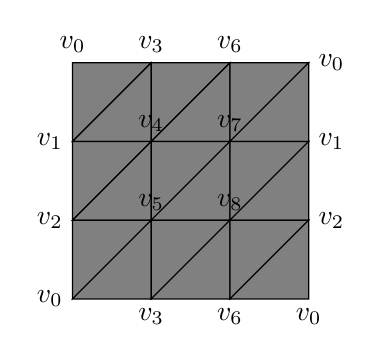
\begin{tikzpicture}
\draw[fill=gray] (0,3) node[anchor=south]{$v_0$} -- (0,2) node[anchor=east]{$v_1$} -- (1,3) -- cycle;
\draw[fill=gray] (0,2) -- (1,3) node[anchor=south]{$v_3$} -- (1,2) -- cycle;
\draw[fill=gray] (1,3) -- (1,2) node[anchor=north]{$v_4$} -- (2,3) node[anchor=south]{$v_6$} -- cycle;
\draw[fill=gray] (1,2) -- (2,3) -- (2,2) -- cycle;
\draw[fill=gray] (2,2) -- (2,3) -- (3,3) node[anchor=west]{$v_0$} -- cycle;
\draw[fill=gray] (2,2) -- (3,3) -- (3,2) node[anchor=west]{$v_1$} -- cycle;
\draw[fill=gray] (0,2) -- (0,1) node[anchor=east]{$v_2$} -- (1,2) node[anchor=south]{$v_4$} -- cycle;
\draw[fill=gray] (0,1) -- (1,2) -- (1,1) node[anchor=north]{$v_3$} -- cycle;
\draw[fill=gray] (1,2) -- (1,1) node[anchor=north]{$v_5$} -- (2,2) -- cycle;
\draw[fill=gray] (1,1) -- (2,2) node[anchor=south]{$v_7$} -- (2,1) -- cycle;
\draw[fill=gray] (2,1) -- (2,2) -- (3,2) -- cycle;
\draw[fill=gray] (2,1) -- (3,2) -- (3,1) node[anchor=west]{$v_2$} -- cycle;
\draw[fill=gray] (0,1) -- (0,0) node[anchor=east]{$v_0$} -- (1,1) node[anchor=south]{$v_5$} -- cycle;
\draw[fill=gray] (0,0) -- (1,1) -- (1,0) node[anchor=north]{$v_3$} -- cycle;
\draw[fill=gray] (1,1) -- (1,0) -- (2,1) -- cycle;
\draw[fill=gray] (1,0) -- (2,1) -- (2,0) node[anchor=north]{$v_6$} -- cycle;
\draw[fill=gray] (2,0) -- (2,1) node[anchor=south]{$v_8$} -- (3,1) -- cycle;
\draw[fill=gray] (2,0) -- (3,1) -- (3,0) node[anchor=north]{$v_0$} -- cycle;
\end{tikzpicture}
\end{figure}
Tomemos $K_1 = \gene{(v_4,v_5,v_7)}$ el complejos generador por el 2-símplice y $K_2 = K \setminus \mathring{K_1}$.
Tenemos que $K_1 \cup K_2 = K$ y $K_1 \cap K_2 = \partial(v_4,v_5,v_7)$.
Sabemos que:
\[ \widetilde{H}_q(K_1 \cap K_2) = \begin{cases}0 & \text{ si }q \neq 1\\\F\gene{z} & \text{ si }q=1\end{cases} \]
Como $K_1$ es un $2$-símplice, $\widetilde{H}_q(K_1) = 0$ para todo $q$.
Para calcular $\widetilde{H}_q(K_2)$, colapsamos el toro con un agujero:
\begin{figure}[H]
\centering
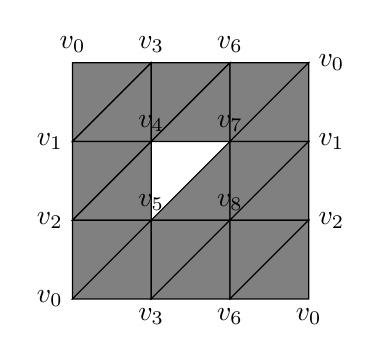
\begin{tikzpicture}
\draw[fill=gray] (0,3) node[anchor=south]{$v_0$} -- (0,2) node[anchor=east]{$v_1$} -- (1,3) -- cycle;
\draw[fill=gray] (0,2) -- (1,3) node[anchor=south]{$v_3$} -- (1,2) -- cycle;
\draw[fill=gray] (1,3) -- (1,2) -- (2,3) node[anchor=south]{$v_6$} -- cycle;
\draw[fill=gray] (1,2) -- (2,3) -- (2,2) -- cycle;
\draw[fill=gray] (2,2) -- (2,3) -- (3,3) node[anchor=west]{$v_0$} -- cycle;
\draw[fill=gray] (2,2) -- (3,3) -- (3,2) node[anchor=west]{$v_1$} -- cycle;
\draw[fill=gray] (0,2) -- (0,1) node[anchor=east]{$v_2$} -- (1,2) node[anchor=south]{$v_4$} -- cycle;
\draw[fill=gray] (0,1) -- (1,2) -- (1,1) node[anchor=north]{$v_5$} -- cycle;
\draw[fill=gray] (1,1) -- (2,2) node[anchor=south]{$v_7$} -- (2,1) -- cycle;
\draw[fill=gray] (2,1) -- (2,2) -- (3,2) -- cycle;
\draw[fill=gray] (2,1) -- (3,2) -- (3,1) node[anchor=west]{$v_2$} -- cycle;
\draw[fill=gray] (0,1) -- (0,0) node[anchor=east]{$v_0$} -- (1,1) node[anchor=south]{$v_5$} -- cycle;
\draw[fill=gray] (0,0) -- (1,1) -- (1,0) node[anchor=north]{$v_3$} -- cycle;
\draw[fill=gray] (1,1) -- (1,0) -- (2,1) -- cycle;
\draw[fill=gray] (1,0) -- (2,1) -- (2,0) node[anchor=north]{$v_6$} -- cycle;
\draw[fill=gray] (2,0) -- (2,1) node[anchor=south]{$v_8$} -- (3,1) -- cycle;
\draw[fill=gray] (2,0) -- (3,1) -- (3,0) node[anchor=north]{$v_0$} -- cycle;
\end{tikzpicture}
\begin{tikzpicture}
\draw (0,1.5) node[anchor=south]{$\searrow\!\!\searrow$};
\draw (0,0) node[anchor=south]{};
\end{tikzpicture}
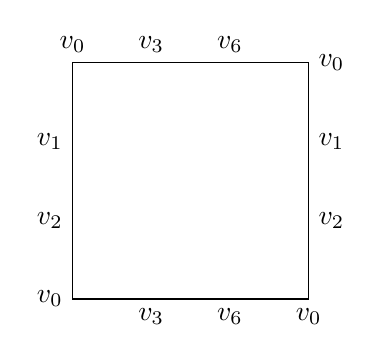
\begin{tikzpicture}
\draw
	(0,3) node[anchor=south]{$v_0$} --
	(0,2) node[anchor=east]{$v_1$} --
	(0,1) node[anchor=east]{$v_2$} --
	(0,0) node[anchor=east]{$v_0$} --
	(1,0) node[anchor=north]{$v_3$} --
	(2,0) node[anchor=north]{$v_6$} --
	(3,0) node[anchor=north]{$v_0$} --
	(3,1) node[anchor=west]{$v_2$} --
	(3,2) node[anchor=west]{$v_1$} --
	(3,3) node[anchor=west]{$v_0$} --
	(2,3) node[anchor=south]{$v_6$} --
	(1,3) node[anchor=south]{$v_3$} --
	cycle;
\end{tikzpicture}
\begin{tikzpicture}
\draw (0,1.5) node[anchor=south]{$=$};
\draw (0,0) node[anchor=south]{};
\end{tikzpicture}
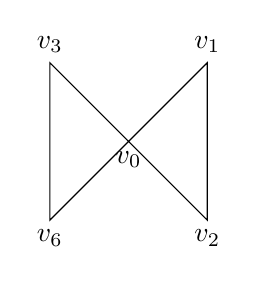
\begin{tikzpicture}
\draw
	(0,2) node[anchor=south]{$v_3$} --
	(0,0) node[anchor=north]{$v_6$} --
	(1,1) node[anchor=north]{$v_0$} --
	(2,2) node[anchor=south]{$v_1$} --
	(2,0) node[anchor=north]{$v_2$} --
	cycle;
\end{tikzpicture}
\begin{tikzpicture}
\draw (0,1.5) node[anchor=south]{$=:L$};
\draw (0,0) node[anchor=south]{};
\end{tikzpicture}
\end{figure}
Luego
\[ \widetilde{H}_q(K_2) \cong H_q(L) = \begin{cases}0 & \text{ si }q\neq 1\\\F^2\gene{\tau_1,\tau_2} & \text{ si }q=1\end{cases}\]
donde
\begin{align*}
\tau_1 & = (v_0,v_6)+(v_6,v_3)+(v_3,v_0)\\
\tau_2 & =(v_0,v_1)+(v_1,v_2)+(v_2,v_0)
\end{align*}
Aplicamos Mayer-Vietoris para $K_1$ y $K_2$:
\begin{align*}
0 & \to \widetilde{H}_2(K_1 \cap K_2) \xrightarrow{i_{*2}} \widetilde{H}_2(K_1)\oplus \widetilde{H}_2(K_2) \xrightarrow{j_{*2}} \widetilde{H}_2(K) \xrightarrow{\Delta_{*2}} \widetilde{H}_1(K_1 \cap K_2) \xrightarrow{i_{*1}}\\
& \xrightarrow{i_{*1}} \widetilde{H}_1(K_1)\oplus \widetilde{H}_1(K_2) \xrightarrow{j_{*1}} \widetilde{H}_1(K) \xrightarrow{\Delta_{*1}} \widetilde{H}_0(K_1 \cap K_2) \xrightarrow{i_{*0}}\\
& \xrightarrow{i_{*0}} \widetilde{H}_0(K_1)\oplus \widetilde{H}_0(K_2) \xrightarrow{j_{*0}} \widetilde{H}_0(K) \to 0
\end{align*}
Con los valores que conocemos:
\begin{align*}
0 & \to 0 \xrightarrow{i_{*2}} 0 \xrightarrow{j_{*2}} \widetilde{H}_2(K) \xrightarrow{\Delta_{*2}} \F\gene{\tau} \xrightarrow{i_{*1}}\\
& \xrightarrow{i_{*1}} \F^2\gene{\tau_1,\tau_2} \xrightarrow{j_{*1}} \widetilde{H}_1(K) \xrightarrow{\Delta_{*1}} 0 \xrightarrow{i_{*0}}\\
& \xrightarrow{i_{*0}} 0 \xrightarrow{j_{*0}} 0 \to 0
\end{align*}
donde $\tau$ es el único $1$-ciclo en $K_1$.
Por exactitud en $\widetilde{H}_1(K_1 \cap K_2)$, tenemos que $\ker i_{*1} = \Ima \Delta_{*2}$.
Veamos que ocurre en $i_{*1}(\tau)$.
Tras dotar a todos los $2$-símplices de una orientación coherente (caras comunes entre símplices inducen orientaciones opuestas), sea:
\[ c = \sum_{\dim(µ \in K_2)=2} µ \]
una $2$-cadena que verifica:
\[ \partial_2(c) = (v_4,v_5)+(v_5,v_7)+(v_7,v_4) = \tau \]
Luego $\tau$ visto en $\widetilde{H}_1(K_2)$ es trivial, por lo que $i_{*1}$ envía $\tau$ en $0$. Así que $\ker i_{*1}=\F\gene{\tau}$. Como $\Delta_{*2}$ es isomorfismo sobre su imagen tenemos que $\widetilde{H}_1(K_2)\cong \Ima\Delta_{*2}\cong \F\gene{\tau}$.

Por otra parte, tenemos que $j_{*1}$ es inyectiva porque hemos probado que $i_{*1}$ es la aplicación nula. Así que por exactitud es de hecho isomorfismo. Esto implica que $\widetilde{H}_1(K)\cong \F^2\gene{\tau_1,\tau_2}$.

Utilizando los cálculos anteriores, $\widetilde{H}_2(K)\cong\Ima\Delta_{*2}=\ker{i_{*1}}\cong\F\gene{\tau}$. Sin embargo podemos escoger un generador más apropiado, basta elegir $c' = \sum_{\dim(µ \in K)=2} µ $, que es un 2-ciclo cuyo borde es 0. 
\end{ej}

\begin{ej}
Sea $K$ la triangulación de la botella de Klein:
\begin{figure}[H]
\centering
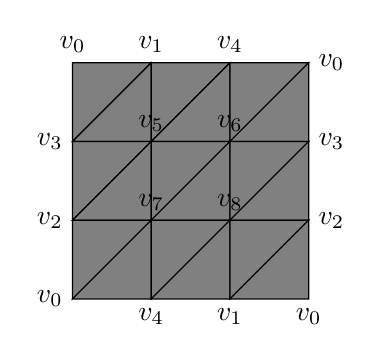
\begin{tikzpicture}
\draw[fill=gray] (0,3) node[anchor=south]{$v_0$} -- (0,2) node[anchor=east]{$v_3$} -- (1,3) -- cycle;
\draw[fill=gray] (0,2) -- (1,3) node[anchor=south]{$v_1$} -- (1,2) -- cycle;
\draw[fill=gray] (1,3) -- (1,2) node[anchor=north]{$v_6$} -- (2,3) node[anchor=south]{$v_4$} -- cycle;
\draw[fill=gray] (1,2) -- (2,3) -- (2,2) -- cycle;
\draw[fill=gray] (2,2) -- (2,3) -- (3,3) node[anchor=west]{$v_0$} -- cycle;
\draw[fill=gray] (2,2) -- (3,3) -- (3,2) node[anchor=west]{$v_3$} -- cycle;
\draw[fill=gray] (0,2) -- (0,1) node[anchor=east]{$v_2$} -- (1,2) node[anchor=south]{$v_5$} -- cycle;
\draw[fill=gray] (0,1) -- (1,2) -- (1,1) node[anchor=north]{$v_3$} -- cycle;
\draw[fill=gray] (1,2) -- (1,1) node[anchor=north]{$v_7$} -- (2,2) -- cycle;
\draw[fill=gray] (1,1) -- (2,2) node[anchor=south]{$v_6$} -- (2,1) -- cycle;
\draw[fill=gray] (2,1) -- (2,2) -- (3,2) -- cycle;
\draw[fill=gray] (2,1) -- (3,2) -- (3,1) node[anchor=west]{$v_2$} -- cycle;
\draw[fill=gray] (0,1) -- (0,0) node[anchor=east]{$v_0$} -- (1,1) node[anchor=south]{$v_7$} -- cycle;
\draw[fill=gray] (0,0) -- (1,1) -- (1,0) node[anchor=north]{$v_4$} -- cycle;
\draw[fill=gray] (1,1) -- (1,0) -- (2,1) -- cycle;
\draw[fill=gray] (1,0) -- (2,1) -- (2,0) node[anchor=north]{$v_1$} -- cycle;
\draw[fill=gray] (2,0) -- (2,1) node[anchor=south]{$v_8$} -- (3,1) -- cycle;
\draw[fill=gray] (2,0) -- (3,1) -- (3,0) node[anchor=north]{$v_0$} -- cycle;
\end{tikzpicture}
\end{figure}

Consideremos $K_1=\{\gene{v_5,v_6,v_7}\}$ y $K_2=K-\{(v_5,v_6,v_7)\}$. Se tiene que $K_1\cup K_2=K$ y $K_1\cap K_2=\partial(v_5,v_6,v_7)$. Procedemos análogamente al ejemplo anterior. Es fácil ver que de nuevo $K_2$ colapsa sobre un wedge de dos circunferencias. Aplicamos Mayer-Vietoris para $K_1$ y $K_2$ con los valores que conocemos:
\begin{align*}
 0 \xrightarrow{j_{*2}} \widetilde{H}_2(K) \xrightarrow{\Delta_{*2}} \F\gene{\tau}
 \xrightarrow{i_{*1}} \F^2\gene{\tau_1,\tau_2} \xrightarrow{j_{*1}} \widetilde{H}_1(K) \xrightarrow{\Delta_{*1}} 0 
\end{align*}
donde $\tau=(v_5,v_6)+(v_6,v_7)+(v_7,v_5)$, $\tau_1=(v_0,v_1)+(v_1,v_4)+(v_4,v_0)$ y $\tau_2=(v_0,v_2)+(v_2,v_3)+(v_3,v_0)$. Veamos cómo funciona $i_{*1}$. Si orientamos $K$ igual que en el ejemplo anterior consideramos 
\[ c = \sum_{\dim(µ \in K_2)=2} µ \]
en $K_2$ se comprueba que $\partial c=\tau+2\tau_1$, por lo que $[\tau]=2[-\tau_1]$ en $H_1(K_2)$. Así que $i_*([\tau])=2[-\tau_1]$ con lo que tenemos que  $i_*$ es inyectiva si la característica de $\F$ no es 2 y nula en caso contrario. Centrémonos en el primer caso. Por exactitud esto implica que $H_2(K)\cong\Ima\Delta_{*2}=\ker i_*=0$. Ahora, usando el primer teorema de isomorfía y la sobreyectividad de $j_{1*}$ tenemos que
\[
H_1(K)\cong \F^2\gene{\tau_1,\tau_2}/2\F\gene{\tau_1}=\F\gene{\tau_2}
\]
por ser $\F$ cuerpo. Además sabemos que $H_0(K)\cong\F\gene{v_0}$ por ser conexo, con lo que hemos terminado. En conclusión, 
$$\widetilde{H}_q(K)\cong \begin{cases}
\F\gene{\tau_2} & q=1\\
0 & c.c.
\end{cases}$$
Si $\F$ es de característica dos, con un procedimiento análogo llegamos a que
$$\widetilde{H}_q(K)\cong \begin{cases}
\F\gene{c'} & q=2\\
\F\gene{\tau_1,\tau_2} & q=1\\
0 & c.c.
\end{cases}$$
donde \[ c' = \sum_{\dim(µ \in K)=2} µ. \]
\end{ej}

\begin{ej}
Sea $K$ la triangulación del plano proyectivo:
\begin{center}
\begin{tikzpicture}[line cap=round,line join=round,>=triangle 45,x=1.0cm,y=1.0cm]
\clip(-0.5,-0.7996279853379787) rectangle (9.22011929968354,3.5);
\draw[fill=gray] (0,0)--(4,0)--(4,3)--(0,3);
\draw (0.,0.)-- (0.,3.);
\draw (0.,3.)-- (4.,3.);
\draw (4.,3.)-- (4.,0.);
\draw (4.,0.)-- (0.,0.);
\draw (2.,3.)-- (2.,2.);
\draw (2.,0.)-- (2.,1.);
\draw (0.,1.5)-- (4.,1.5);
\draw (1.5,1.5)-- (0.,3.);
\draw (0.,3.)-- (2.,2.);
\draw (2.,2.)-- (4.,3.);
\draw (2.5,1.5)-- (4.,3.);
\draw (1.5,1.5)-- (0.,0.);
\draw (0.,0.)-- (2.,1.);
\draw (2.,1.)-- (4.,0.);
\draw (2.5,1.5)-- (4.,0.);
\draw (1.5,1.5)-- (2.,2.);
\draw (1.5,1.5)-- (2.,1.);
\draw (2.,1.)-- (2.5,1.5);
\draw (2.5,1.5)-- (2.,2.);
\draw (4.129392345695879,3.1982774400655742) node[anchor=north west] {$v_0$};
\draw (1.85268082781231,3.4714828222116028) node[anchor=north west] {$v_3$};
\draw (-0.6,3.1800637479225053) node[anchor=north west] {$v_2$};
\draw (-0.6,1.6956478382624167) node[anchor=north west] {$v_1$};
\draw (-0.6,0.183911390387725) node[anchor=north west] {$v_0$};
\draw (1.9437492885276526,-0.04375976140063218) node[anchor=north west] {$v_3$};
\draw (4.156712883910482,0.183911390387725) node[anchor=north west] {$v_2$};
\draw (4.147606037838948,1.7138615304054852) node[anchor=north west] {$v_1$};
\draw (2.,2.55) node[anchor=north west] {$v_4$};
\draw (2.2,2) node[anchor=north west] {$v_5$};
\draw (1.2,1.9688532204084452) node[anchor=north west] {$v_6$};
\draw (2.,0.9488864603966051) node[anchor=north west] {$v_7$};
\end{tikzpicture}
\end{center}

Tomamos $K_1=\gene{v_4,v_5,v_6}$ y $K_2=K-\{(v_4,v_5,v_6)\}$. Ya conocemos la homología de $K_1$. Es fácil ver que $K_2$ colapsa sobre el ciclo de vértices $v_0,v_1,v_2,v_3$, al que denotaremos $\tau$, que ya hemos probado que su homología es la misma que la de cualquier otra triangulación de $S^1$. Además, $K_1\cap K_2=\partial(v_4,v_5,v_6)=\sigma$. Así, en Mayer-Vietoris reducida obtenemos
\[
0\xrightarrow{}H_2(K)\xrightarrow{\Delta_{*2}}\F\gene{\sigma}  \xrightarrow{i_{*1}}\F\gene{\tau}\xrightarrow{j_{*1}} H_1(K) \xrightarrow{} 0 
\]
Si orientamos $K$ igual que en el ejemplo anterior consideramos 
\[ c = \sum_{\dim(µ \in K_2)=2} µ \]
en $K_2$ se comprueba que $\partial c=\sigma+2\tau$, por lo que $[\sigma]=2[-\tau]$ en $H_1(K_2)$. Así que $i_*([\sigma])=2[-\tau]$ con lo que tenemos que  $i_*$ es inyectiva si $\F$ no es de característica 2. Por exactitud esto implica que $H_2(K)\cong\Ima\Delta_{*2}=\ker i_*=0$. Ahora, usando el primer teorema de isomorfía y la sobreyectividad de $j_{1*}$ tenemos que
\[
H_1(K)\cong \F\gene{\tau}/2\F\gene{\tau}=0
\]
por ser $\F$ cuerpo. En conclusión, $\widetilde{H}_q(K)=0$ para todo $q$. Si $\F$ fuera de característica 2, entonces $\ker{i_*}=\F\gene{\tau}$. En este caso, $H_2(K)\cong \F\gene{\tau}$ (aunque podemos tomar como generador la suma de los 2-símplices) y $H_1(K)\cong\F\gene{\tau}$.
\end{ej}

En el siguiente capítulo probaremos que los cálculos de los ejemplos anteriores son válidos para cualquier otra triangulación que se realice de los espacios en cuestión.

\end{document}